\providecommand{\main}{..}

\documentclass[\main/main]{subfiles}

\setcounter{chapter}{4}

\begin{document}

\tableofcontents

\chapter{Exploration in MDPs}

\section{Introduction}

In the chapter on fitted DP \eqref{ch:fitted_dp}, we explored algorithms for finding the optimal value and policy in an MDP when the transition and reward functions are unknown.
However, we swept the issue of \emph{exploration} under the hood.
Namely, our algorithms might easily \emph{overfit} to certain areas of the state space,
missing out on possible better paths.
This issue is especially relevant in \textbf{sparse reward} problems where reward might not be achieved until after many steps,
and algorithms which do not \emph{systematically} explore new states may entirely fail to learn anything meaningful.

For example, policy gradient algorithms require \emph{signal} in the gradient to learn. In other words, if we never observe any reward, the gradient will always be zero, and the policy will never improve.

\begin{example}{Sparse Reward MDP}{sparse_reward_mdp}
    Here's a simple example of an MDP with sparse reward:

    \begin{center}
        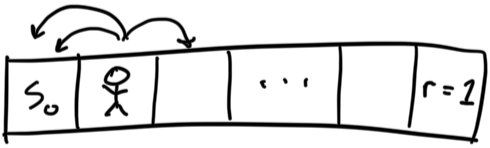
\includegraphics{sparse_reward_mdp}
    \end{center}

    There are $|\S|$ states.
    The agent starts in the leftmost state. There are three possible actions, two of which move the agent left and one which moves the agent right. The reward function assigns $r=1$ to the rightmost cell.
\end{example}

How can we address this issue?

Let's start by assuming that the MDP is \emph{deterministic}, that is, taking action $a$ in state $s$ will always take you to the state $P(s, a) \in \S$. We will save issues of randomness for later.

Then, one algorithm to trade off exploration and exploitation is:

\begin{enumerate}
    \item \textbf{Explore:} Visit every possible state-action pair to fully understand the MDP.
    \item \textbf{Exploit:} Now the MDP is fully known, so we can use a planning algorithm like policy iteration \eqref{df:pi_iter} to solve for the optimal policy.
\end{enumerate}

\begin{definition}{Explore-then-exploit (for deterministic MDPs)}{explore_then_exploit}
    We'll keep a set $K$ of all the $(s, a, r, s')$ pairs we've observed.
    Each episode, we'll choose an unseen pair $(s, a)$ for which the reward $r(s, a)$ and the next state $s' = P(s, a)$ are unknown, and take the shortest path there.

    \begin{algorithmic}
        \State $K \gets \emptyset$
        \While{$\exists (s, a)$ s.t. there is no $(s, a, r, s') \in K$}
        \State Using our known transitions $K$, compute the shortest path to $(s, a)$
        \State Take the shortest path to $(s, a)$
        \State $K \gets K \cup \{ (s, a) \}$
        \EndWhile
        \State Compute the optimal policy $\pi^\star$ in the MDP $K$ (e.g. using policy iteration).
        \State \Return $\pi^\star$.
    \end{algorithmic}

    We leave it to the reader to design an efficient implementation of the shortest-path algorithm.
\end{definition}

\begin{theorem}{Performance of explore-then-exploit}{explore_then_exploit_performance}
    As long as every state can be reached from $s_0$ within a single episode, i.e. $|\S| \le \hor$, this will eventually be able to explore all $|\S| |\A|$ state-action pairs, adding one new transition per episode/trajectory.

    We can measure the performance using the \textbf{regret} across episodes. That is, let $K_t$ denote the value of $K$ at iteration $t$, and let us compare the value of the optimal policy $\pi_t$ derived from $K_t$ with the value of the \emph{true} optimal policy $\pi^\star$.

    As we described above, we know that it will take at most $SA$ iterations to explore the entire MDP, after which $\pi_t = \pi^\star$.
    For the $\pi_t$ up until then, however, we can construct a very loose bound as follows.
    At each interaction, the reward from $\pi_t$ might differ from $\pi^\star$ by at most $1$.
    Since an episode is $\hor$ steps long, this means the value of policy $\pi_t$ will differ from that of $\pi^\star$ by at most $\hor$.
    So,
    \[
        \sum_{t=1}^T V_0(\pi^\star) - V_0(\pi_t) \le |\S||\A| \hor.
    \]
\end{theorem}

\section{Treating an unknown MDP as a MAB}

We also explored the exploration-exploitation tradeoff in the chapter on multi-armed bandits \eqref{ch:1_bandits}.
Recall the overall framework of MAB:
We have $K$ arms, each of which has an unknown reward distribution,
and we want to learn which of the arms is \emph{optimal}, i.e. gives the highest mean reward.

One algorithm that struck a good balance between exploration and exploitation was the \textbf{upper confidence bound} algorithm \eqref{df:ucb},
where for each arm we construct a \emph{confidence interval} for its true mean award, and then choose the arm that achieves the highest upper confidence bound on its mean reward. In summary,
\[k_{t+1} \gets \argmax_{k \in [K]} \frac{S^{k}_t}{N^{k}_t} + \sqrt{\frac{\ln(2t/\delta)}{2 N^{k}_t}}\]
where $N_t^k$ indicates the number of times arm $k$ has been pulled up until time $t$,
$S_t^k$ indicates the total reward obtained by pulling arm $k$ up until time $t$,
and $\delta > 0$ controls the width of the confidence interval.
How might we extend UCB to the MDP case?

Let us formally describe an unknown MDP as an MAB problem.
In an unknown MDP, we want to learn which \emph{policy} is optimal. So if we want to apply MAB techniques to solving an MDP, it makes sense to think of \emph{arms} as \emph{policies}.
This gives us $(|\A|^{\S})^\hor$ arms for deterministic policies in a finite MDP.
Then, ``pulling'' arm $\pi$ corresponds to using $\pi$ to act through a trajectory in the MDP, and observing the total reward.

\begin{exercise}
    Which quantity that we have seen so far equals the mean reward from arm $\pi$?
\end{exercise}

Recall that UCB incurs regret $\tilde{O}(\sqrt{TK})$, where $T$ is the number of pulls and $K$ is the number of arms.
Substituting in the values above, we see that treating policies as arms and running UCB incurs regret
\[
    \tilde{O}(|\A|^{|\S|\hor/2} N)
\]
where $N$ is the number of trajectories we get to observe.
This scales \emph{exponentially} in $|\S|$ and $\hor$, which quickly becomes intractable.
Notably, this method doesn't consider the information that we gain across different policies. We can illustrate this with the following example:

\begin{example}{Treating an MDP as a MAB is ineffective}{ineffective_mdp}
    Consider a ``coin MDP'' with two states ``heads'' and ``tails'', two actions ``Y'' and ``N'', and a time horizon of $\hor=2$.
    The state transition flips the coin, and doesn't depend on the action.
    The reward only depends on the action: Taking action Y gives reward $1$, and taking action N gives reward $0$.

    Suppose we collect a data from the two constant policies $\pi_{\text{Y}}(s) = \text{Y}$ and $\pi_{\text{N}}(s) = \text{N}$.
    Now we want to learn about policy $\tilde{\pi}$ that takes action Y and then N.
    Do we need to collect data about $\tilde{\pi}$?
    No! We can infer its behaviour on timestep $1$ from our data on policy $\pi_{\text{Y}}$ and its behaviour on timestep $2$ from our data on policy $\pi_{\text{N}}$.
    But if we treat the MDP as a bandit, we treat $\tilde{\pi}$ as a new arm about which we know nothing.
\end{example}

\section{UCB-VI}

One way to frame the UCB algorithm is that, when choosing arms, we optimize over a \emph{proxy reward} that is the sum of the estimated mean reward and an exploration term.

Can we extend this idea to the case of an unknown MDP $\mathcal{M}^{?}$? That is, can we model a proxy MDP $\tilde{\mathcal{M}}$ with a reward function that encourages exploration, and then use DP to solve for the optimal policy in $\tilde{\mathcal{M}}$?
This brings us to the \textbf{UCB-VI} algorithm.

\textbf{Assumptions:} For simplicity, here we assume the reward function of $M_{?}$ is known, so we only need to model the state transitions. We will consider the more general case of a \textbf{time-varying} MDP, where the transition and reward functions can change over time. We take the convention that $P_\hi$ is the distribution of $s_{h+1} \mid s_{h}, a_{h}$ and $r_\hi$ is applied to $s_\hi, a_\hi$.

\begin{definition}{UCB-VI}{ucb_vi}
For $t \in [T]$:
\begin{enumerate}
    \item \textbf{Modelling:} We use previous data to model the transitions $\hat{P}_0, \dots, \hat{P}_{H-2}$. We design a reward bonus $b_\hi(s, a) \in \R$ to encourage exploration, analogous to the UCB term.
    \item \textbf{Optimistic planning:} Using DP, We solve for the optimal policy $\pi_\hi$ in the modelled MDP \[ \tilde{M} = (\S, \A, \{ \hat{P}_\hi \}_{h \in [H-1]}, \{ r_\hi + b_\hi \}_{h \in [H-1]}, H). \] Then we use $\pi_\hi$ to collect a new trajectory, and repeat.
\end{enumerate}
\end{definition}

Note that the bonuses also \emph{propagate backwards} via the DP algorithm.
This effectively enables us to \emph{plan to explore} unknown states.

We detail each of these steps below.

\subsection{Modeling the transitions}

Let $\mathcal{D}_\hi^t$ denote the dataset of transitions collected at timestep $h$ from the first $t$ trajectories. That is, $\mathcal{D}_\hi^t = \{ s_\hi^i, a_\hi^i, s_{h+1}^i \}_{i \in [t]}$.

We seek to approximate $P_\hi(s_{h+1} \mid s_\hi, a_\hi) = \frac{\P(s_\hi, a_\hi, s_{h+1})}{\P(s_\hi, a_\hi)}$. We can estimate these using their sample probabilities from the dataset. That is, define
\begin{align*}
    N_\hi^t(s, a, s') &:= \sum_{i=0}^{t-1} \mathbf{1}\{ s_\hi^i = s, a_\hi^i = a, s_{h+1}^i = s' \} \\
    N_\hi^t(s, a) &:= \sum_{s' \in \S} N_\hi^t(s, a, s') \\
\end{align*}
Then we can model
\[
    \hat{P}_\hi^t(s' \mid s, a) = \frac{N_\hi^t(s, a, s')}{N_\hi^t(s, a)}.
\]
\begin{remark}
Note that this is also a fairly naive estimate, and doesn't assume any underlying structure of the MDP. Thus it would be considered a \emph{nonparametric} model. We'll see how to improve this in the following section, and use underlying structure to improve our estimates.
\end{remark}

\subsection{Reward bonus}

To motivate the reward bonus term $b_\hi^t(s, a)$, recall how we designed the reward bonus term for UCB:
\begin{enumerate}
    \item  We used Hoeffding's inequality to bound, with high probability, how far the sample mean $\hat \mu_k^t$ deviated from the true mean $\mu_k$.
    \item By inverting this inequality, we obtained a $(1-\delta)$-confidence interval for the true mean,
    centered at our estimate.
    \item To make this bound \emph{uniform} across all timesteps $t \in [T]$,
    we applied the union bound and multiplied $\delta$ by a factor of $T$.
\end{enumerate}

We'd like to do the same for UCB-VI, and construct the bonus term such that $V_\hi^\star \le \hat{V}_\hi^t(s)$ with high probability.
However, our construction will be more complex than the MAB case, since $\hat{V}_\hi^t(s)$ depends on $b_\hi^t(s, a)$ implicitly via the DP algorithm.
We claim that the bonus term that satisfies this property is
\[
    b_\hi^t(s, a) = 2 H \sqrt{\frac{\log( |\S||\A|H T/\delta )}{N_\hi^t(s, a)}}.
\]
We will only provide a heuristic sketch of the proof; see \cite[Section 7.3]{agarwal_reinforcement_2022} for a full proof.

\begin{derivation}{UCB-VI reward bonus construction}{ucb_vi_bonus}
    We aim to show that, with high probability, \[
        V_\hi^\star(s) \le \hat{V}_\hi^t(s) \quad \forall t \in [T], h \in [H].
    \]
    We'll do this by bounding the error incurred at each step of DP. Recall that DP solves for $\hat{V}_\hi^t(s)$ recursively as follows:
    \[
        \hat{V}_\hi^t(s) = \max_{a \in \A} \left[ \tilde r^t_\hi(s, a) + \E_{s' \sim \hat{P}_\hi^t(\cdot \mid s, a)} \left[ \hat{V}_{h+1}^t(s') \right] \right]
    \]
    where $\tilde r^t_\hi(s, a) = r_\hi(s, a) + b_\hi^t(s, a)$ is the reward function of our modelled MDP $\tilde{M}^t$.
    There are two possible sources of error:
    \begin{enumerate}
        \item The value functions $\hat{V}^t_{h+1}$ v.s. $\Vopt_{h+1}$
        \item The transition probabilities $\hat{P}_\hi^t$ v.s. $P^?_\hi$.
    \end{enumerate}
    For the former, we can simply bound the difference by $H$, assuming that the rewards are within $[0, 1]$. Now, all that is left is to bound the error from the transition probabilities, and we can combine these two bounds with the triangle inequality.
    
    First, for a fixed $s, a, h, t$, we aim to bound the error caused by the state transitions:
    \begin{equation}
        \text{error} = \left| \E_{s' \sim \hat{P}_\hi^t(\cdot \mid s, a)} \left[ \Vopt_{h+1}(s') \right] - \E_{s' \sim P^?_\hi(\cdot \mid s, a)} \left[ \Vopt_{h+1}(s') \right]. \right|
        \label{eq:err}
    \end{equation}

    Note that expanding out the definition of $\hat{P}_\hi^t$ gives
    \begin{align*}
        \E_{s' \sim \hat{P}_\hi^t(\cdot \mid s, a)} \left[ \Vopt_{h+1}(s') \right] &= \sum_{s' \in \S} \frac{N^t_\hi(s, a, s')}{N^t_\hi(s, a)} \Vopt_{h+1}(s') \\
        &= \frac{1}{N^t_\hi(s, a)} \sum_{i=0}^{t-1} \sum_{s' \in \S} \mathbf{1}\{ (s_\hi^i, a_\hi^i, s_{h+1}^i) = (s, a, s') \} \Vopt_{h+1}(s') \\
        &= \frac{1}{N^t_\hi(s, a)} \sum_{i=0}^{t-1} \underbrace{\mathbf{1}\{ (s_\hi^i, a_\hi^i) = (s, a) \} \Vopt_{h+1}(s_{h+1}^i)}_{X^i}
    \end{align*}
    since the terms where $s' \neq s_{h+1}^i$ vanish.

    Now, in order to apply Hoeffding's inequality, we would like to express the second term in \eqref{eq:err} as a sum over $t$ random variables as well. We will do this by redundantly averaging over all desired trajectories (i.e. where we visit state $s$ and action $a$ at time $h$):
    \begin{align*}
        \E_{s' \sim P^?_\hi(\cdot \mid s, a)} \left[ \Vopt_{h+1}(s') \right]
        &= \sum_{s' \in \S} P^?_\hi(s' \mid s, a) \Vopt_{h+1}(s') \\
        &= \sum_{s' \in \S} \frac{1}{N^t_\hi(s, a)} \sum_{i=0}^{t-1} \mathbf{1}\{ (s_\hi^i, a_\hi^i) = (s, a) \} P^?_\hi(s' \mid s, a) \Vopt_{h+1}(s') \\
        &= \frac{1}{N^t_\hi(s, a)} \sum_{i=0}^{t-1} \E_{s_{h+1}^i \sim P^?_{h}(\cdot \mid s_\hi^i, a_\hi^i)} X^i.
    \end{align*}
    Now we can apply Hoeffding's inequality to obtain that, with probability at least $1-\delta$,
    \[
        \text{error} = \left| \frac{1}{N^t_\hi(s, a)} \sum_{i=0}^{t-1} \left(X^i - \E_{s_{h+1}^i \sim P^?_{h}(\cdot \mid s_\hi^i, a_\hi^i)} X^i \right) \right| \le 2 H \sqrt{\frac{\ln(1/\delta)}{N_\hi^k(s, a)}}.
    \]
    Applying a union bound over all $s \in \S, a \in \A, t \in [T], h \in [H]$ gives the $b_\hi^t(s, a)$ term above.
\end{derivation}

\subsection{Performance of UCB-VI}

How exactly does UCB-VI strike a good balance between exploration and exploitation? In UCB, the bonus exploration term was fairly interpretable, but now we must consider the value function of the policy returned by UCB-VI at iteration $t$, that is, $V^{\pi^t}_\hi(s)$.

Recall we constructed $b^t_\hi$ so that, with high probability, $\Vopt_\hi(s) \le \hat{V}_\hi^t(s)$ and so \[
    \Vopt_\hi(s) - V^{\pi^t}_\hi(s) \le \hat{V}_\hi^t(s) - V^{\pi^t}_\hi(s).
\]
If the r.h.s. is \emph{small}, this implies that the l.h.s. difference is also small, i.e. that $\pi^t$ is \emph{exploiting} actions that are giving high reward.

If the r.h.s. is \emph{large}, then we have overestimated the value: $\pi^t$, the optimal policy of $\tilde{M}$, does not perform well in the true environment $M^?$. This indicates that either some $b_\hi^t(s, a)$ must be large, which corresponds to an action taken to \emph{explore} the environment, or some $\hat P^t_\hi(\cdot \mid s, a)$ is inaccurate; but notice that this correlates with a low visit count of $(s, a)$, and thus $b_\hi^t(s, a)$ being large.

It turns out that UCB-VI achieves a per-episode regret of
\[
    \E \left[ \sum_{t=0}^{T-1} \left(\Vopt_0(s_0) - V^{\pi^t}_0(s_0) \right) \right] = \tilde{O}(H^2 \sqrt{|\S| |\A| T})
\]
Comparing this to the UCB regret bound $\tilde{O}(\sqrt{T K})$,
we see that we've reduced the number of effective arms from 

For some more intuition, consider how many episodes it takes for us to achieve an average regret of $1$. Ignoring the $H^2$ factor (we'll see later why this is allowed), the average regret is
\[
    \frac{1}{T} \E[\text{Regret}_T] = \tilde{O}\left(\sqrt{\frac{|\S||\A|}{T}}\right),
\]
and for this to be constant, it would take $T = \Omega(|\S||\A|)$ steps.
Note the number of entries of the $\Qopt$ matrix is of the same order.
But note that the transition matrix has $|\S|^2 |\A|$ entries.
This shows that it's possible to achieve low regret, and achieve a near-optimal policy, while only understanding a $1/|\S|$ fraction of the world.

\todo{Discussion of $H^2$ term}

\section{Linear MDPs}

Above, when estimating the transition matrix $\hat P^t_\hi$, we said that we can do in the case where we don't know anything about the structure of the MDP.
But in many cases, for large or continuous $|\S|$ and $|\A|$, even some polynomial factor in $|\S|$ and $|\A|$ will become intractable.
Instead, we're going to look at \textbf{linear MDPs}: an example of a \emph{parameterized} MDP where the rewards and state transitions depend only on some \emph{low-dimensional} parameter space.

\begin{definition}{Linear MDP}{linear_mdp}
    We assume that the transition probabilities and rewards are \emph{linear} in some feature vector $\phi(s, a) \in \R^d$:
    \begin{align*}
        P_\hi(s' \mid s, a) &= \phi(s, a)^\top \mu^\star_\hi(s') \\
        r_\hi(s, a) &= \phi(s, a)^\top \theta_\hi^\star
    \end{align*}
    Note that we can also think of $P_\hi(\cdot \mid s, a) = \mu_\hi^\star$ as an $|\S| \times d$ matrix, and think of $\mu^\star_\hi(s')$ as indexing into the $s'$-th row of this matrix (treating it as a column vector). Thinking of $\Vopt$ as an $|\S|$-dimensional vector, this allows us to write \[ \E_{s' \sim P_\hi(\cdot \mid s, a)}[\Vopt(s)] = (\mu^\star_\hi \phi(s, a))^\top \Vopt. \]
    The $\phi$ feature mapping could be designed to capture interactions between the state $s$ and action $a$.
    In this book, we'll assume that the feature map $\phi : \S \times \A \to \R^d$ and the reward $\theta_\hi^\star$ are known.
\end{definition}

Let's see what value iteration looks like in a linear MDP.

\subsection{UCB-VI in a linear MDP}

First, value iteration can be described as follows:

We initialize $V_{H}^\star(s) = 0 \forall s$. Then we iterate:

\begin{align*}
    \Qopt_\hi(s, a) &= r_\hi(s, a) + \E_{s' \sim P_\hi(\cdot \mid s, a)} [\Vopt_{h+1}(s')] \\
    &= \phi(s, a)^\top \theta_\hi^\star + (\mu_\hi^\star \phi(s, a))^\top \Vopt_{h+1} \\
    &= \phi(s, a)^\top \underbrace{( \theta_\hi^\star + (\mu_\hi^\star)^\top  \Vopt_{h+1})}_{w_\hi} \\
    \Vopt_\hi(s) &= \max_a \Qopt_\hi(s, a) \\
    \pi^\star_\hi(s) &= \argmax_a \Qopt_\hi(s, a)
\end{align*}

Now, we can use techniques from \textbf{supervised learning} to model the unknown MDP.

Let us write $\delta_s \in \S$ as a one-hot vector in $\R^{|\S|}$, with a $1$ in the $s$-th entry and $0$ everywhere else.
Note that \[
\E_{s' \sim P_h(\cdot \mid s, a)} [\delta_{s'}] = P_h(\cdot \mid s, a) = \mu_h^\star \phi(s, a).
\]
Recall that \textbf{supervised learning} is precisely useful for estimating conditional expectations by minimizing mean squared error. Furthermore, since the expectation here is linear in terms of (some function of) the observed quantities $s, a$, we can directly apply least-squares multi-target linear regression (with a regularization term) to construct the estimate
\[
\hat \mu = \argmin_{\mu \in \R^{|\S| \times d}} \sum_{t=0}^{T-1} \|\mu \phi(s_h^i, a_h^i) - \delta_{s_{h+1}^i} \|_2^2 + \lambda \|\mu\|_{\text{F}}^2.
\]
This has a well-known closed-form solution:
\begin{align*}
    \hat \mu^\top &= (A_h^t)^{-1} \sum_{i=0}^{t-1} \phi(s_h^i, a_h^i) \delta_{s_{h+1}^i}^\top \\
    \text{where} \quad A_h^t &= \sum_{i=0}^{t-1} \phi(s_h^i, a_h^i) \phi(s_h^i, a_h^i)^\top + \lambda I
\end{align*}

We can directly plug in this estimate into $\hat{P}^t_h(\cdot \mid s, a) = \hat \mu^t_h \phi(s, a)$.

Now, to design the reward bonus, we can't apply Hoeffding anymore, since the terms no longer involve sample means of bounded random variables; instead, we're incorporating information across different states and actions. Rather, we can construct an upper bound using \emph{Chebyshev's inequality}.

\end{document}


